\noindent S~myšlienkou využívať digitálne počítače na preklad
prirodzených jazykov prišiel v~roku 1946 A. D. Booth a~uchytila sa aj
vďaka značnej finančnej podpore tejto oblasti v~50. a~80. rokoch 20.
storočia. Napriek tomu sa \underbar{strojovému prekladu} nepodarilo
splniť očakávania, ktoré naň boli kladené už v~začiatočných
rokoch po jeho vzniku.

Strojový preklad jednoducho nahrádza slová jedného prirodzeného
jazyka slovami iného jazyka. To sa dá využiť v~oblastiach s~veľmi
obmedzeným, stereotypným jazykom, akým je napríklad jazyk predpovede
počasia. Pre dobrý preklad menej štandardizovaných textov však
treba pričleniť väčšie textové celky (frázy, vety alebo dokonca
celé pasáže) k~ich najbližším náprotivkom v~cieľovom jazyku.
Hlavný problém tkvie vo fakte, že ľudský jazyk je dvojznačný.
Jazyková dvojznačnosť prináša problémy na mnohých jazykových
úrovniach, napríklad \underbar{viacznačnosť slovných významov} na
lexikálnej rovine („Leopard“ môže znamenať zviera alebo
operačný systém) alebo pripojenie atribútov na syntaktickej rovine
ako v~príkladoch:

\begin{verse}
{\em Otcovi priatelia neprišli, moji áno.}\\
\smallskip
{\em Otcovi priatelia neprišli, mne áno.}
\end{verse}

Jeden z~možných prístupov k~problému sa zakladá na lingvistických
pravidlách. Pre preklad medzi blízko príbuznými jazykmi (ako však aj
už uvedených príkladoch) je prípustná aj metóda priameho prekladu.
Takéto systémy založené na pravidlách analyzujú vstupný text
a~vytvárajú „prostredníka“, symbolickú reprezentáciu, z~ktorej
sa generuje text cieľového jazyka. Úspech týchto metód veľmi
závisí od dostupnosti rozsiahlych lexikónov
s~morfologickými, syntaktickými a~sémantickými údajmi a~aj
s~veľkými súbormi \underbar{gramatických} pravidiel vypracovaných
skúsenými lingvistami. 

\begin{figure*}[htb]
  \colorrule{grey3}{\textwidth}{1.5pt}
  \center
  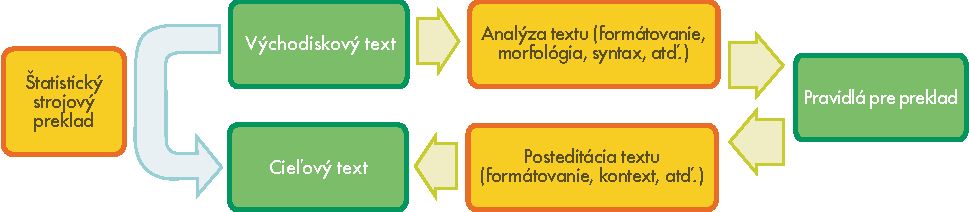
\includegraphics[width=\textwidth]{../_media/slovak/machine_translation}
  \caption{Strojový preklad (štatistický; založený na pravidlách)}
  \label{fig:mtarch_sk}
  \colorrule{grey3}{\textwidth}{1.5pt}
\end{figure*}

Koncom 80. rokov 20. storočia, teda v~čase, keď sa počítače
začali rozmáhať a~stali sa cenovo dostupnejšie, zvýšil sa záujem
o~štatistické modely pre strojový preklad. Parametre týchto
štatistických modelov sú odvodené z~analýzy bilingválneho
textového korpusu, akým je aj paralelný korpus Europarl,
ktorý obsahuje rokovania Európskeho parlamentu v~21 európskych
jazykoch. Ak dostane štatistický strojový preklad dostatok údajov,
funguje dostatočne dobre na to, aby odvodil približný význam
cudzieho jazyka v~texte. Na rozdiel od systémov riadených znalosťami
však štatistický (alebo dátami riadený) strojový preklad často
generuje gramaticky nesprávne výstupy. Na druhej strane však okrem
zníženej potreby ľudského úsilia na pravopisné písanie dokáže
strojový preklad riadený dátami pokryť také špecifiká jazyka,
akými sú napríklad idiomatické výrazy, ktoré zas chýbajú
v~systémoch riadených vedomosťami. 

Keďže sa silné a~slabé stránky strojového prekladu riadeného
vedomosťami a~strojového prekladu riadeného dátami navzájom
dopĺňajú, v~súčasnosti sa vedci usilujú kombinovaním oboch metód
uplatniť hybridné postupy. To je uskutočniteľné mnohými spôsobmi.
Jedným z~nich je možnosť použiť oba typy systémov a~nechať
rozhodnúť výberový modul o~najvhodnejšom výstupe pre každú vetu.
Pre dlhšie vety však nebude dokonalý žiadny výsledok. Lepším
riešením je preto skombinovanie najlepších častí každej vety
z~viacerých výstupov, čo však môže byť značne zložité, keďže
korešpondujúce časti rozličných alternatív nie sú vždy
zrozumiteľné a~musia byť nanovo usporiadané. 

V~90. rokoch 20. storočia bol navrhnutý prototyp strojového prekladu
medzi blízko príbuznou češtinou a~slovenčinou na Karlovej univerzite
v~Prahe.

TEOS Trenčín uviedol na trh prvý praktický mnohojazyčný softvér
strojového prekladu pre slovenský jazyk spolu s~ich PC slovníkovým
softvérom. Keďže však systém nepoužíval nijakú hlbšiu
lingvistickú analýzu a~jednoducho nahrádzal slová jedného jazyka
slovami druhého jazyka (zväčša obmedzené len na lemy), jeho
uplatnenie sa obmedzovalo len na jazyky, ktoré nedisponujú bohatým
morfologickým systémom, t.j. na angličtinu. Novšie verzie vedia
prekladať webové stránky za behu, čo je funkcia mimoriadne
užitočná pre anglicko-slovenské preklady (zároveň jediný
fungujúci smer prekladu).


Kvalita systémov strojového prekladu disponuje stále obrovským
potenciálom na zlepšenie. Súčasné výzvy spočívajú hlavne
v~adaptabilite jazykových zdrojov na danú doménu alebo
používateľskú oblasť a~v~ich integrácii do existujúceho
pracovného toku výrazových základní a~prekladových pamätí.
Väčšina súčasných systémov (nielen tých orientovaných na
slovenský jazyk) je orientovaná na angličtinu. Najvyššiu kvalitu
prekladu z/do angličtiny ponúka predovšetkým Google Translate. 

\boxtext{Kvalita systémov strojového prekladu disponuje stále obrovským potenciálom na zlepšenie}

Dostupnosť veľkého množstva bilingválnych textov je v~štatistickom
strojovom preklade skutočne kľúčová. Pre slovenčinu sa
v~súčasnosti korpus paralelných textov spolu s~mnohými inými
jazykmi len buduje. Najviac dát -- spolu milióny párov viet -- je
dostupných v~slovensko-českom a~slovensko-anglickom paralelnom
korpuse, ktorý sa zostavuje v~Jazykovednom ústave Ľ. Štúra. Obsah
korpusu tvorí prevažne beletria a~vety sú automaticky zarovnané.
